\section{Gedächtniss}
\begin{itemize}
	\item Die mentale Fähigkeit, Informationen zu enkodieren, zu speichern, zu konsolidieren und abzurufen 
	\item Enkodeieren: Prozess, bei dem eine mentale Repräsentation der Information erstellt wird
	\item Speicherung: Übertragung \& Behalten der repräsentierten Informationen im Gedächtnis
	\item Konsolidierung: Stabilisierung der Information im Gedächtnis
	\item Abruf: Die Aktivierung gespeicherter Informationen im Gedächtnis 
\end{itemize}
\subsection{Explizites vs. implizites Gedächtnis}
\begin{itemize}
	\item Implizites Gedächtnis:
		\begin{itemize}
			\item Informationen sind aus dem Gedächtnis verfügbar, ohne bewusstes Enkodieren oder Abrufen
		\end{itemize}
	\item Explizites Gedächtnis: 
		\begin{itemize}
			\item Enkodierung und Abruf brauchen Aufmerksamkeit, mentale Anstrengung und sind bewusst
		\end{itemize}
	\item Deklaratives Gedächtnis:
		\begin{itemize}
			\item Fakten und Ereignisse, die man sprachlich wiedergeben kann
		\end{itemize}
	\item Nondeklaratives Gedächtndis:
		\begin{itemize}
			\item Repräsentationen, die sich im Verhalten ausdrücken, aber nicht sprachlich berichtbar sind
			\item z.B. prozedurales Gedächtnis für Motorik
		\end{itemize}
\end{itemize}
\subsection{Explizite Gedächtnisstrukturen und -prozesse}
\subsubsection{Drei-Speicher Modell}
\begin{center}
	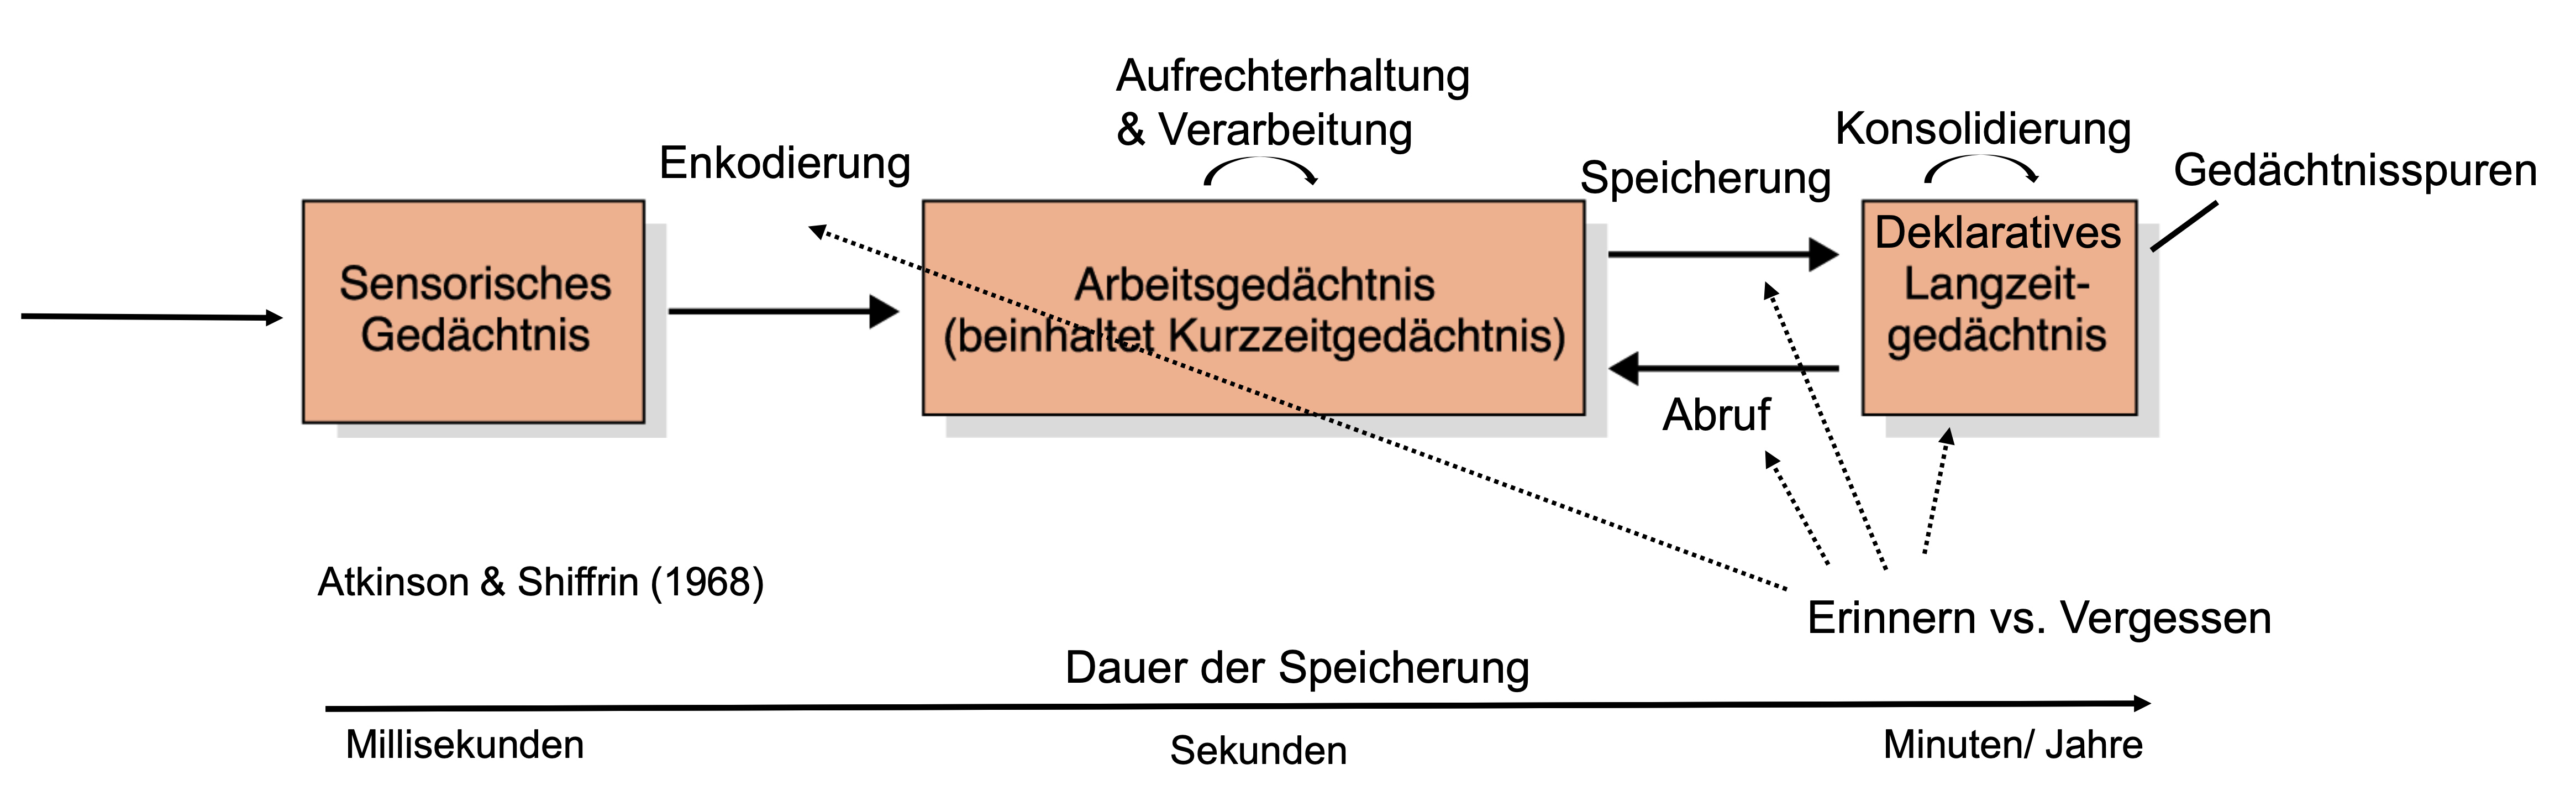
\includegraphics[scale=.2]{img/Drei_Speicher.png}
\end{center}
\subsubsection{Strukturen im Langzeitgedächtnis}
\begin{center}
	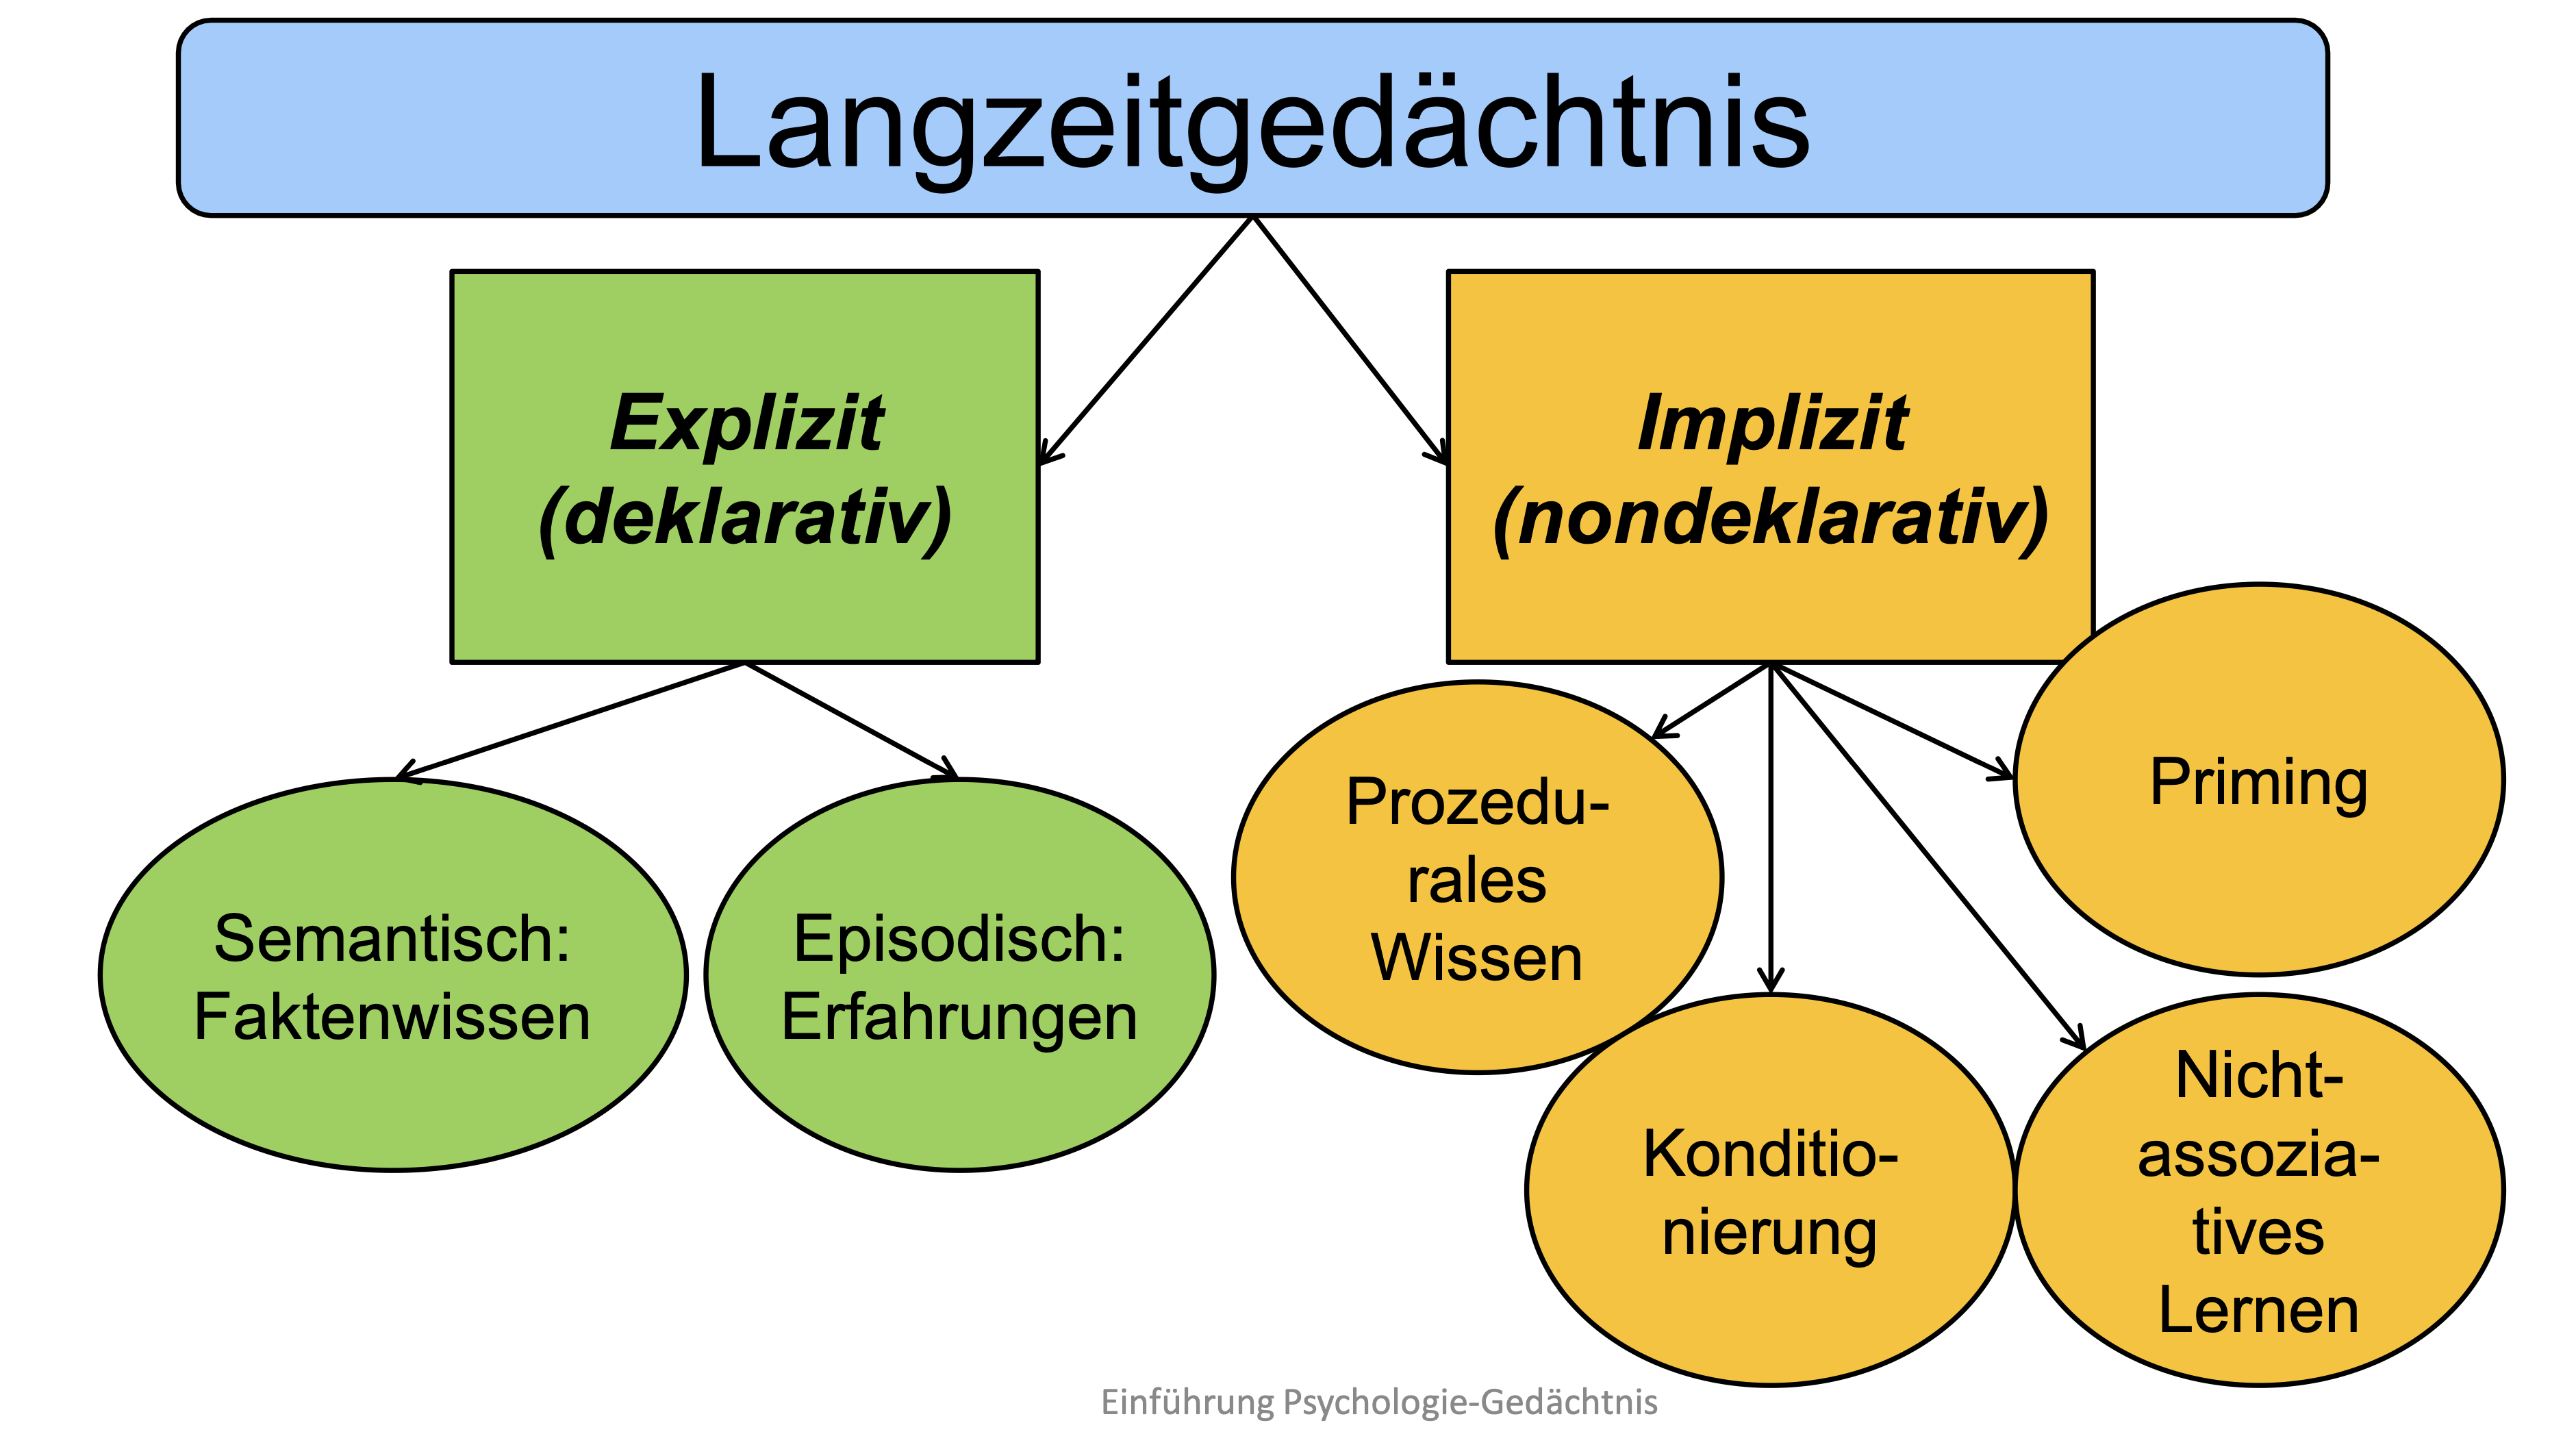
\includegraphics[scale=.2]{img/Langzeitgedaechtnis.png}
\end{center}
\subsubsection{Sensorisches Gedächtnis}
\begin{itemize}
	\item Ikonisches Gedächtnis:
		\begin{itemize}
			\item Sensorisches Gedächtnis für visuelle Informationen, speichert große Informationsmengen für sehr kurze Dauer (<500 ms)  
		\end{itemize}
	\item Echoisches Gedächtnis:
		\begin{itemize}
			\item Sensrisches Gedächtnis für auditive Informationen, speichert mit kurzer Dauer (<4 s) 
		\end{itemize}	
\end{itemize}
\subsubsection{Kurzzeitgedächtnis}
\begin{itemize}
	\item KZG: Gedächtnisprozesse, die die Repräsentation kürzlich enkodierter Erfahrungen aufrecht erhalten und Informationen aus dem Langzeitgedächtnis abrufen
	\item KGZ hat begrenzte Kapazität ($7\pm2$ Items) und speichert Informationen nur kurze Zeit (15-20 s)
	\item Trotz begrenzter Kapazität kommen wir im Alltag gut zurecht, dank:
		\begin{itemize}
			\item Rehearsal: Aufrechterhaltung durch mentale Wiederholung
			\item Chunking: Zusammenfassung in größere Sinneinheiten (chunks)
		\end{itemize}
\end{itemize}
\subsubsection{Arbeitsgedächtnis}
\begin{itemize}
	\item Arbeitsgedächtnis speichert und manipuliert mit begrenzter Kapazität Informationen für komplexe Aufgabenwie Verstehen, Lernen und Schlussfolgern
\end{itemize}
\subsubsection{Langzeitgeächtnis}
\begin{itemize}
	\item Assoziativität und Inhaltsadressierbarkeit:
		\begin{itemize}
			\item Abruf durch Hinweisreize (retrieval cues), die als Teil der Gedächtnisspur die gesamte Gedächtnisspur im LZG aktivieren
		\end{itemize}
	\item 2 Formen des expliziten Abrufs:
		\begin{itemize}
			\item Passives Wiedererkennen (recall)
			\item Aktiver Abruf (recall): Stimulus muss reproduziert werden
		\end{itemize}
	\item Enkodierspezifität:
		\begin{itemize}
			\item Abruf von Information wird in dem Maße besser, in dem die Hinweisreize beim Abruf mit den Umgebungsreizen beim Enkodieren übereinstimmen
		\end{itemize}
\end{itemize}
\subsubsection{Vergessen}
\begin{itemize}
	\item Vergessen: Verlust von Erinnerungen über die Zeit
	\item Interferenz: Ähnliche Gedächtnisspuren von alten und neuen Gedächtnisinhalten überlagern sich \rightarrow schlechterer Abruf von neuen und alten Inhalten 
\end{itemize}
\subsection{Neuronale Grundlagen des Gedächtnisses}
\begin{center}
	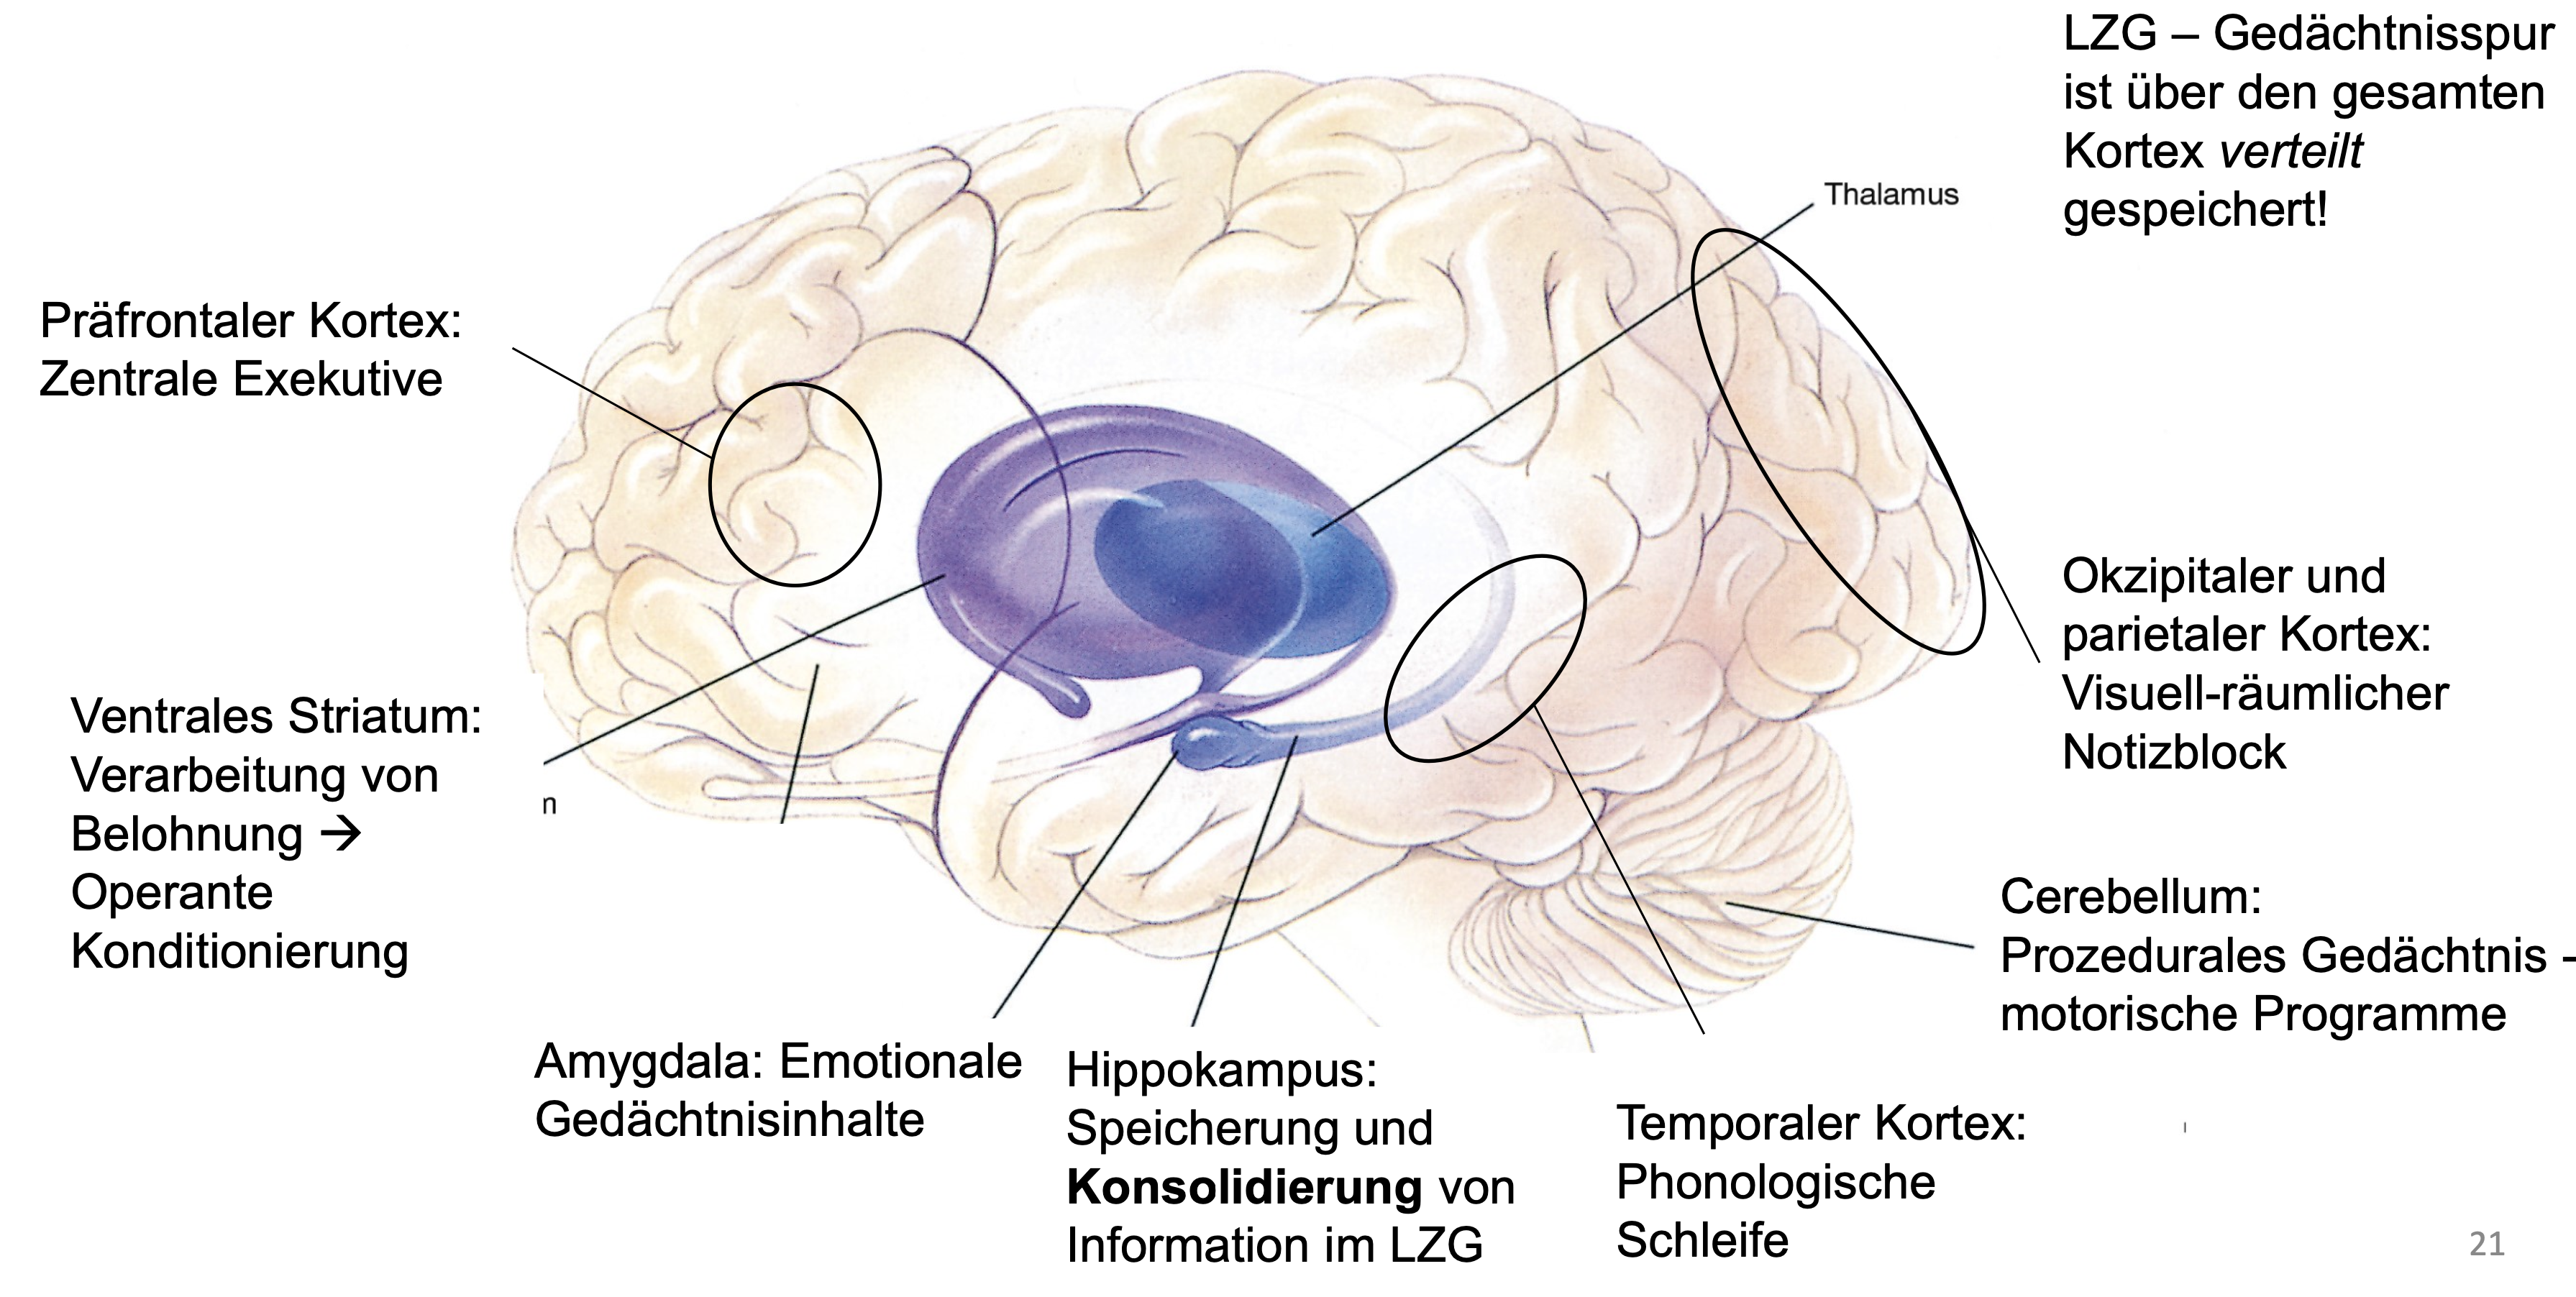
\includegraphics[scale=.2]{img/Gedeachtnis_Gehrin.png}
\end{center}
\subsubsection{Amnesien}
\begin{itemize}
	\item Anterograde vs. Retrograde Amnesie
		\begin{itemize}
			\item Anterograd: Unfähigkeit, neue Informationen nach Trauma/Krankheit zu speichern
			\item Retrograd: Unfähigkeit alte Informationen vor dem Trauma/Krankheit abzurufen
		\end{itemize}
	\item Amnesie bei
		\begin{itemize}
			\item Hirnschädigung: Entfernung des Hippokampus \rightarrow anterorage Amnesie mit intaktem KZG
			\item Demenzen, z.B. Alzheimer: Ablagerung von plaques beginnend im Hippokampus \rightarrow beide Arten der Amnesie
		\end{itemize}
\end{itemize}


